\documentclass[11pt,a4paper]{article}
\usepackage[margin=1in]{geometry}
\usepackage[utf8]{inputenc}
\usepackage[T1]{fontenc}
\usepackage{tikz}
\usepackage{amsmath}
\usepackage[round]{natbib}
\usetikzlibrary{arrows.meta,positioning,shapes,decorations.pathreplacing}

\title{HMC vs Gibbs Sampling}
\author{}
\date{\today}

\begin{document}

\maketitle

\section{Hamiltonian Monte Carlo (HMC)}

\subsection{Overview}

Figure~\ref{fig:hmc-visual} shows the geometry of one HMC iteration in parameter space. We start at our current position $\theta^{(t)}$ (the blue point), introduce momentum $p$ (the blue arrow), and then simulate Hamiltonian dynamics guided by the gradient $\nabla \log p(\theta|y)$ (the green arrow). This creates a curved trajectory (the blue path) that proposes a new point $\theta^{\text{proposal}}$ (the orange point). Finally, we accept or reject this proposal using a Metropolis step.

\begin{figure}[htbp]
\centering
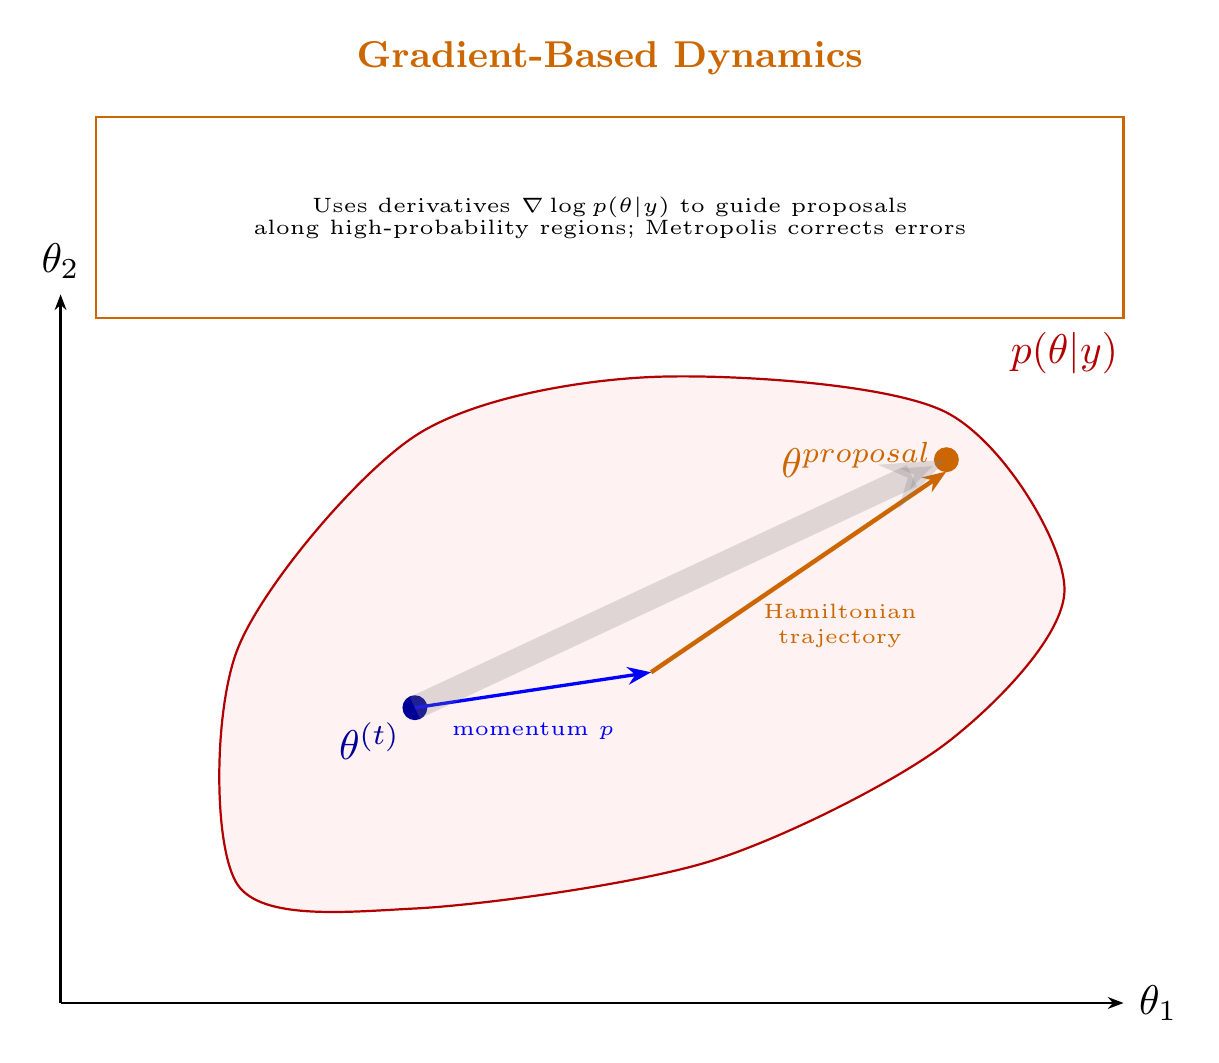
\begin{tikzpicture}[scale=1.5, transform shape]
    % Draw axes
    \draw[-{Stealth[length=2mm]}, thick] (0,0) -- (9,0) node[right] {$\theta_1$};
    \draw[-{Stealth[length=2mm]}, thick] (0,0) -- (0,6) node[above] {$\theta_2$};
    
    % Draw posterior contour (transparent)
    \draw[thick, red!70!black, draw=red!70!black, fill=red!5] plot[smooth cycle] coordinates {
        (1.5,1) (3,0.8) (5.5,1.2) (7.5,2.2) (8.5,3.5) (7.5,5) (5,5.3) (3,4.8) (1.5,3)
    };
    \node[red!70!black] at (8.5,5.5) {$p(\theta|y)$};
    
    % Starting point
    \fill[blue!60!black] (3,2.5) circle (3pt);
    \node[below left, blue!60!black] at (3,2.5) {$\theta^{(t)}$};
    
    % Momentum vector
    \draw[-{Stealth[length=3mm]}, blue, very thick] (3,2.5) -- (5,2.8);
    \node[blue, below, font=\tiny] at (4,2.5) {momentum $p$};
    
    % Hamiltonian trajectory (straight line) - starts from momentum endpoint
    \draw[orange!80!black, ultra thick, -{Stealth[length=3mm]}] (5,2.8) -- (7.5,4.5);
    \node[below, font=\tiny, orange!80!black, align=center] at (6.6,3.5) {Hamiltonian\\trajectory};
    
    % Proposed point
    \fill[orange!80!black] (7.5,4.6) circle (3pt);
    \node[left, orange!80!black] at (7.5,4.6) {$\theta^{proposal}$};
    
    % Wide transparent arrow from theta^(t) to theta^proposal (drawn on top)
    \draw[-{Stealth[length=8mm]}, line width=3mm, opacity=0.25, gray] (3,2.5) -- (7.5,4.6);
    
    % Title well above plot area
    \node[orange!80!black, font=\small\bfseries] at (4.65,8.0) {Gradient-Based Dynamics};
    
    % Annotation box with better vertical spacing
    \draw[thick, orange!80!black] (0.3,5.8) rectangle (9,7.5);
    \node[font=\tiny, align=center] at (4.65,6.65) {
        Uses derivatives $\nabla \log p(\theta|y)$ to guide proposals\\[-0.1em]
        along high-probability regions; Metropolis corrects errors
    };
\end{tikzpicture}
\caption{HMC visual summary: current position, momentum, gradient direction, and Hamiltonian trajectory leading to a proposal.}
\label{fig:hmc-visual}
\end{figure}

The key idea behind HMC is to use auxiliary variables—extra variables not part of the original model that help the algorithm work more efficiently. Specifically, HMC adds momentum variables $p$ and then simulates Hamiltonian dynamics, treating parameters as positions and momentum as velocities according to physics-inspired equations. This simulation uses the derivative of the log posterior $\nabla \log p(\theta|y)$, which tells us how the posterior probability changes as we move through parameter space. We compute the derivative with respect to each parameter (the partial derivative $\partial \log p(\theta|y) / \partial \theta_j$) to guide the trajectory towards high-probability regions. Finally, a Metropolis accept--reject step corrects for numerical errors in the simulation, ensuring the sampler converges to the correct posterior distribution (a property called detailed balance).

\subsection{Walking Through One HMC Iteration}

We now walk through one iteration of HMC step by step, showing the notation, the variables that exist at each stage, and how they connect to the diagram in Figure~\ref{fig:hmc-visual}.

\subsubsection*{Step 0: Setup and notation}

Before we begin sampling, we define our model and prior. For example:
$$
p(\theta) \quad \text{with} \quad \beta \sim \mathcal{N}(0, 100).
$$
Our target is the posterior distribution:
$$
p(\theta|y) \propto p(y|\theta) p(\theta).
$$
We start at the previous sample $\theta^{(n-1)}$. This is the blue point $\theta^{(t)}$ in Figure~\ref{fig:hmc-visual}. At this stage, we have just one vector:
\begin{itemize}
    \item $\theta^{(n-1)}$ (56 parameter values)
\end{itemize}

\subsubsection*{Step 1: Sample momentum}

HMC introduces auxiliary momentum variables $p$ drawn independently from:
$$
p_0 \sim \mathcal{N}(0, I).
$$
This is the blue arrow labelled ``momentum $p$'' in Figure~\ref{fig:hmc-visual}. Setting $\theta_0 = \theta^{(n-1)}$, we now have two vectors:
\begin{itemize}
    \item $\theta_0 = \theta^{(n-1)}$ (56 parameter values)
    \item $p_0$ (56 momentum values)
\end{itemize}

In code, this looks like:
\begin{verbatim}
theta <- theta_start
p     <- rnorm(length(theta), mean = 0, sd = 1)
\end{verbatim}

\subsubsection*{Step 2: Leapfrog trajectory}

Starting from $(\theta_0, p_0)$, we apply $L$ leapfrog updates. Each update alternates between a half-step momentum update using the gradient $\nabla \log p(\theta|y)$ (the green arrow in Figure~\ref{fig:hmc-visual}), a full-step position update, and another half-step momentum update. This creates the sequence:
$$
(\theta_0, p_0) \rightarrow (\theta_1, p_1) \rightarrow \cdots \rightarrow (\theta_L, p_L).
$$
The curved blue path in Figure~\ref{fig:hmc-visual} represents this Hamiltonian trajectory. During the trajectory, we have intermediate states $(\theta_k, p_k)$ for $k=0,\ldots,L$, but we only keep the endpoint. After the trajectory completes, we have four vectors:
\begin{itemize}
    \item $\theta^{(n-1)} = \theta_0$ (56 starting parameter values)
    \item $p_0$ (56 starting momentum values)
    \item $\theta_L$ (56 new parameter values after $L$ steps)
    \item $p_L$ (56 updated momentum values after $L$ steps)
\end{itemize}

In code:
\begin{verbatim}
for (k in 1:L) {
    grad  <- grad_log_posterior(theta, y)
    p     <- p + 0.5 * eps * grad
    theta <- theta + eps * p
    grad  <- grad_log_posterior(theta, y)
    p     <- p + 0.5 * eps * grad
}
\end{verbatim}

\subsubsection*{Step 3: Proposal}

We set the proposal to be the endpoint of the trajectory:
\begin{align*}
\theta^{\text{proposal}} &= \theta_L \\
p^{\text{proposal}} &= p_L
\end{align*}
This is the orange point $\theta^{\text{proposal}}$ in Figure~\ref{fig:hmc-visual}. We still have the same four vectors as before, just relabelled:
\begin{itemize}
    \item $\theta^{(n-1)}$ (56 starting values)
    \item $p_0$ (56 starting momentum values)
    \item $\theta^{\text{proposal}}$ (56 proposed new values)
    \item $p^{\text{proposal}}$ (56 final momentum values)
\end{itemize}

In code:
\begin{verbatim}
theta_proposal <- theta
\end{verbatim}

\subsubsection*{Step 4: Accept or reject}

We compute the log acceptance probability:
$$
\log \alpha = \log p(\theta^{\text{proposal}}|y) - \log p(\theta^{(n-1)}|y).
$$
Then we accept the proposal with probability $\min(1, e^{\log \alpha})$:
$$
\theta^{(n)} = 
\begin{cases}
\theta^{\text{proposal}} & \text{with probability } \min(1, e^{\log \alpha}) \\
\theta^{(n-1)} & \text{otherwise}
\end{cases}
$$
This Metropolis step corrects for numerical errors from the leapfrog approximation. After this step, the momentum values are discarded (they were auxiliary), and we have just one vector:
\begin{itemize}
    \item $\theta^{(n)}$ (56 parameter values for the next iteration)
\end{itemize}

In code:
\begin{verbatim}
log_post_prop <- log_posterior(theta_proposal, y)
log_post_curr <- log_posterior(theta_start, y)
log_alpha     <- log_post_prop - log_post_curr

if (log(runif(1)) < log_alpha) {
    theta_next <- theta_proposal
} else {
    theta_next <- theta_start
}
\end{verbatim}

\subsubsection*{Step 5: Repeat}

We return to Step 1 with $\theta^{(n-1)} = \theta^{(n)}$ and continue sampling.

\clearpage

\section{Blocked Gibbs Sampling}

\subsection{Overview}

Figure~\ref{fig:gibbs-visual} shows the geometry of one blocked Gibbs iteration. We start at our current position $\theta^{(t)}$ (the blue point), which contains all parameters $(\beta, u, \tau_e, \tau_u)$. Unlike HMC, which uses gradients and momentum, Gibbs sampling updates parameters sequentially by sampling from full conditional distributions. Each parameter (or block of parameters) is updated by drawing from its conditional distribution given all other parameters and the data. The three coloured arrows show the three moves: sampling $\tau_u$ (blue vertical arrow), sampling $(\beta, u)$ jointly (green horizontal arrow), and sampling $\tau_e$ (purple vertical arrow), arriving at $\theta^{(t+1)}$ (the purple point).

\begin{figure}[htbp]
\centering
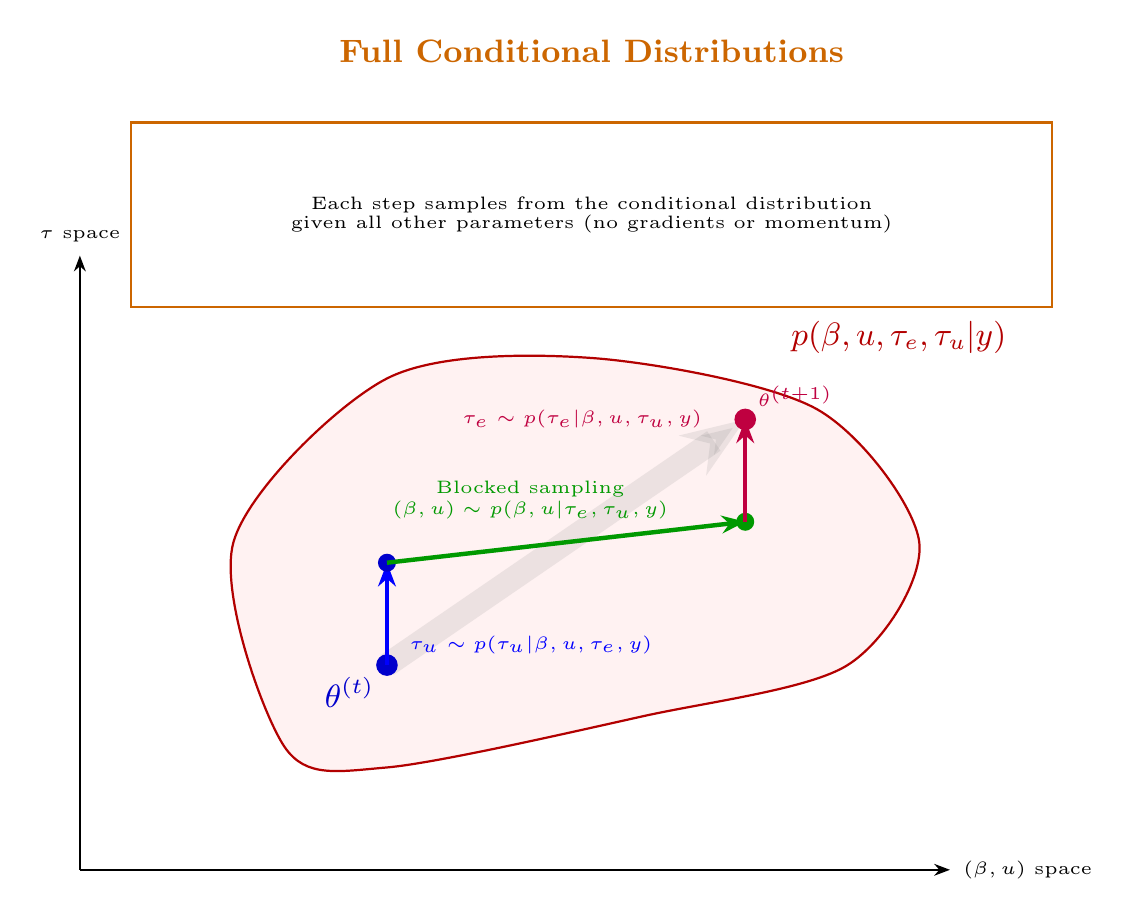
\begin{tikzpicture}[scale=1.3, transform shape]
    % Draw axes
    \draw[-{Stealth[length=2mm]}, thick] (0,0) -- (8.5,0) node[right, font=\tiny] {$(\beta, u)$ space};
    \draw[-{Stealth[length=2mm]}, thick] (0,0) -- (0,6) node[above, font=\tiny] {$\tau$ space};
    
    % Draw posterior contour (very light fill)
    \draw[thick, red!70!black, fill=red!5] plot[smooth cycle] coordinates {
        (2,1.2) (3,1) (5.5,1.5) (7.5,2) (8.2,3.2) (7.2,4.5) (5,5) (3,4.8) (1.5,3.2)
    };
    \node[red!70!black, font=\small] at (8,5.2) {$p(\beta, u, \tau_e, \tau_u | y)$};
    
    % Wide transparent arrow from theta^(t) to theta^(t+1)
    \draw[-{Stealth[length=8mm]}, line width=3mm, opacity=0.15, gray] (3,2) -- (6.5,4.4);
    
    % Starting point
    \fill[blue!80!black] (3,2) circle (3pt);
    \node[below left, blue!80!black, font=\small] at (3,2) {$\theta^{(t)}$};
    
    % Step 1: Sample tau_u (vertical move in tau space)
    \draw[-{Stealth[length=3mm]}, blue, ultra thick] (3,2) -- (3,3);
    \node[right, blue, align=left, font=\tiny] at (3.1,2.2) {$\tau_u \sim p(\tau_u|\beta,u,\tau_e,y)$};
    \fill[blue!80!black] (3,3) circle (2.5pt);
    
    % Step 2: Sample (beta, u) jointly
    \draw[-{Stealth[length=3mm]}, green!60!black, ultra thick] (3,3) -- (6.5,3.4);
    \node[above, green!60!black, align=center, font=\tiny] at (4.4,3.3) {Blocked sampling\\$(\beta,u) \sim p(\beta,u|\tau_e,\tau_u,y)$};
    \fill[green!60!black] (6.5,3.4) circle (2.5pt);
    
    % Step 3: Sample tau_e (vertical move in tau space)
    \draw[-{Stealth[length=3mm]}, purple, ultra thick] (6.5,3.4) -- (6.5,4.4);
    \node[left, purple, align=right, font=\tiny] at (6.2,4.4) {$\tau_e \sim p(\tau_e|\beta,u,\tau_u,y)$};
    \fill[purple] (6.5,4.4) circle (3pt);
    \node[above right, purple, font=\tiny] at (6.5,4.4) {$\theta^{(t+1)}$};
    
    % Title well above plot area
    \node[orange!80!black, font=\small\bfseries] at (5,8.0) {Full Conditional Distributions};
    
    % Annotation box for full conditionals with better vertical spacing
    \draw[thick, orange!80!black] (0.5,5.5) rectangle (9.5,7.3);
    \node[font=\tiny, align=center] at (5,6.4) {
        Each step samples from the conditional distribution\\[-0.1em]
        given all other parameters (no gradients or momentum)
    };
    
\end{tikzpicture}
\caption{Blocked Gibbs sampling: three sequential updates via full conditional distributions.}
\label{fig:gibbs-visual}
\end{figure}

The key idea behind Gibbs sampling is to use full conditional distributions—the probability distribution of one parameter (or block of parameters) conditional on all others and the data. These distributions often have closed-form expressions, allowing direct sampling without gradients, momentum variables, or acceptance steps. For variance components $\tau_e$ and $\tau_u$, the full conditionals are typically inverse-gamma distributions. For the regression parameters $(\beta, u)$ given the variances, the full conditional is a multivariate normal. By cycling through these conditionals, the sampler explores the joint posterior without ever computing derivatives.

\subsection{Walking Through One Gibbs Iteration}

We now walk through one iteration of blocked Gibbs sampling step by step, showing the notation, the variables that exist at each stage, and how they connect to the diagram in Figure~\ref{fig:gibbs-visual}.

\subsubsection*{Step 0: Setup and notation}

Our hierarchical model is:
\begin{align*}
y &= X\beta + Zu + \varepsilon, \quad \varepsilon \sim \mathcal{N}(0, \tau_e^{-1} I) \\
u &\sim \mathcal{N}(0, \tau_u^{-1} K)
\end{align*}
where $\theta = (\beta, u, \tau_e, \tau_u)$ contains all parameters. Our target is the posterior:
$$
p(\beta, u, \tau_e, \tau_u | y) \propto p(y | \beta, u, \tau_e) p(u | \tau_u) p(\beta) p(\tau_e) p(\tau_u).
$$
Note that each hyperparameter appears twice: $\tau_e$ appears in the likelihood $p(y|\beta,u,\tau_e)$ and in its own prior $p(\tau_e)$; similarly, $\tau_u$ appears in the conditional prior for $u$ and in its own prior. This structure is characteristic of Bayesian hierarchical models, where hyperparameters govern lower-level distributions whilst themselves being treated as random variables with their own priors~\cite{gelman2006data,gelman2006prior}.

We start at the previous sample $\theta^{(t)} = (\beta^{(t)}, u^{(t)}, \tau_e^{(t)}, \tau_u^{(t)})$. This is the blue point in Figure~\ref{fig:gibbs-visual}. At this stage, we have:
\begin{itemize}
    \item $\beta^{(t)}$ (4 values)
    \item $u^{(t)}$ (50 values)
    \item $\tau_e^{(t)}$ (1 value)
    \item $\tau_u^{(t)}$ (1 value)
\end{itemize}
Total: 56 parameter values in $\theta^{(t)}$.

\subsubsection*{Step 1: Sample $\tau_u$}

We sample the random effect variance component from its full conditional:
$$
\tau_u^{(t+1)} \sim p(\tau_u | \beta^{(t)}, u^{(t)}, \tau_e^{(t)}, y).
$$
For our model, this is an inverse-gamma distribution:
$$
\tau_u^{(t+1)} \sim \text{InvGamma}\left(a_u + \frac{n_u}{2}, \, b_u + \frac{1}{2} u^{(t)T} K^{-1} u^{(t)}\right).
$$
This is the blue vertical arrow in Figure~\ref{fig:gibbs-visual}, moving in $\tau$ space whilst holding $(\beta, u)$ fixed. After this step, we have:
\begin{itemize}
    \item $\beta^{(t)}$ (4 values, unchanged)
    \item $u^{(t)}$ (50 values, unchanged)
    \item $\tau_e^{(t)}$ (1 value, unchanged)
    \item $\tau_u^{(t+1)}$ (1 new value)
\end{itemize}

In code:
\begin{verbatim}
shape_u <- a_u + n_u / 2
rate_u  <- b_u + 0.5 * t(u) %*% solve(K) %*% u
tau_u   <- rgamma(1, shape = shape_u, rate = rate_u)
\end{verbatim}

\subsubsection*{Step 2: Sample $(\beta, u)$ jointly}

We sample the regression parameters and random effects jointly from their full conditional:
\begin{align*}
(\beta^{(t+1)}, u^{(t+1)}) &\sim p(\beta, u | \tau_e^{(t)}, \tau_u^{(t+1)}, y)
\end{align*}
For our model, this is a multivariate normal distribution. The joint update (blocked sampling) is crucial for good mixing when $\beta$ and $u$ are correlated. This is the green horizontal arrow in Figure~\ref{fig:gibbs-visual}, moving in $(\beta, u)$ space whilst holding $(\tau_e, \tau_u)$ fixed. After this step, we have:
\begin{itemize}
    \item $\beta^{(t+1)}$ (4 new values)
    \item $u^{(t+1)}$ (50 new values)
    \item $\tau_e^{(t)}$ (1 value, unchanged)
    \item $\tau_u^{(t+1)}$ (1 value from Step 1)
\end{itemize}

In code:
\begin{verbatim}
# Precision matrix for joint (beta, u)
Q       <- tau_e * t(cbind(X, Z)) %*% cbind(X, Z)
Q[5:54, 5:54] <- Q[5:54, 5:54] + tau_u * solve(K)

# Mean vector
mu      <- solve(Q) %*% (tau_e * t(cbind(X, Z)) %*% y)

# Sample jointly
theta   <- mvrnorm(1, mu = mu, Sigma = solve(Q))
beta    <- theta[1:4]
u       <- theta[5:54]
\end{verbatim}

\subsubsection*{Step 3: Sample $\tau_e$}

We sample the error variance component from its full conditional:
$$
\tau_e^{(t+1)} \sim p(\tau_e | \beta^{(t+1)}, u^{(t+1)}, \tau_u^{(t+1)}, y).
$$
For our model, this is an inverse-gamma distribution:
$$
\tau_e^{(t+1)} \sim \text{InvGamma}\left(a_e + \frac{n}{2}, \, b_e + \frac{1}{2} (y - X\beta^{(t+1)} - Zu^{(t+1)})^T (y - X\beta^{(t+1)} - Zu^{(t+1)})\right).
$$
This is the purple vertical arrow in Figure~\ref{fig:gibbs-visual}, moving in $\tau$ space whilst holding $(\beta, u, \tau_u)$ fixed. After this step, we arrive at $\theta^{(t+1)}$ (the purple point), and we have:
\begin{itemize}
    \item $\beta^{(t+1)}$ (4 values from Step 2)
    \item $u^{(t+1)}$ (50 values from Step 2)
    \item $\tau_e^{(t+1)}$ (1 new value)
    \item $\tau_u^{(t+1)}$ (1 value from Step 1)
\end{itemize}
Total: 56 parameter values in $\theta^{(t+1)}$.

In code:
\begin{verbatim}
resid    <- y - X %*% beta - Z %*% u
shape_e  <- a_e + n / 2
rate_e   <- b_e + 0.5 * sum(resid^2)
tau_e    <- rgamma(1, shape = shape_e, rate = rate_e)
\end{verbatim}

\subsubsection*{Step 4: Repeat}

We return to Step 1 with $\theta^{(t)} = \theta^{(t+1)}$ and continue sampling.

\subsection{Key Differences from HMC}

\begin{itemize}
    \item No gradients: Gibbs samples directly from full conditionals; HMC uses $\nabla \log p(\theta|y)$ to guide trajectories
    \item No auxiliary variables: Gibbs updates parameters in place; HMC introduces momentum $p$
    \item No accept/reject: Gibbs always accepts (samples are exact from conditionals); HMC uses Metropolis correction
    \item Sequential updates: Gibbs cycles through parameter blocks; HMC updates all parameters jointly via the trajectory
    \item Closed-form sampling: Gibbs relies on tractable conditionals (inverse-gamma, multivariate normal); HMC works even when conditionals are intractable
\end{itemize}

Both methods explore the posterior $p(\theta|y)$, but via completely different mechanisms. Gibbs is simpler when conditionals are available, whilst HMC is more robust to correlations and scales better to high dimensions.

\bibliographystyle{plainnat}
\bibliography{../../report/references}

\end{document}
